\documentclass[red]{tutorial}
\usepackage[no-math]{fontspec}
\usepackage{xpatch}
	\renewcommand{\ttdefault}{ul9}
	\xpatchcmd{\ttfamily}{\selectfont}{\fontencoding{T1}\selectfont}{}{}
	\DeclareTextCommand{\nobreakspace}{T1}{\leavevmode\nobreak\ }
\usepackage{polyglossia} % English please
	\setdefaultlanguage[variant=us]{english}
%\usepackage[charter,cal=cmcal]{mathdesign} %different font
%\usepackage{avant}
\usepackage{microtype} % Less badboxes

%\usepackage{enumitem}

\usepackage[charter,cal=cmcal]{mathdesign} %different font
%\usepackage{euler}
 
\usepackage{blindtext}
\usepackage{calc, ifthen, xparse, xspace}
\usepackage{makeidx}
\usepackage[hidelinks, urlcolor=blue]{hyperref}   % Internal hyperlinks
\usepackage{mathtools} % replaces amsmath
\usepackage{bbm} %lower case blackboard font
\usepackage{amsthm, bm}
\usepackage{thmtools} % be able to repeat a theorem
\usepackage{thm-restate}
\usepackage{graphicx}
\usepackage[dvipsnames]{xcolor}
\usepackage{multicol}
\usepackage{fnpct} % fancy footnote spacing
\usepackage{tikz}
\usetikzlibrary{arrows.meta}

\usepackage{pgfplots}
\pgfplotsset{compat=1.18}
%\pgfkeys{/pgf/fpu}

 
\newcommand{\xh}{{{\mathbf e}_1}}
\newcommand{\yh}{{{\mathbf e}_2}}
\newcommand{\zh}{{{\mathbf e}_3}}
\newcommand{\R}{\mathbb{R}}
\newcommand{\Z}{\mathbb{Z}}
\newcommand{\N}{\mathbb{N}}
\newcommand{\proj}{\mathrm{proj}}
\newcommand{\Proj}{\mathrm{proj}}
\newcommand{\Perp}{\mathrm{perp}}
\renewcommand{\span}{\mathrm{span}\,}
\newcommand{\Span}{\mathrm{span}\,}
\newcommand{\Img}{\mathrm{img}\,}
\newcommand{\Null}{\mathrm{null}\,}
\newcommand{\Range}{\mathrm{range}\,}
\newcommand{\rref}{\mathrm{rref}}
\newcommand{\rank}{\mathrm{rank}}
\newcommand{\Rank}{\mathrm{rank}}
\newcommand{\nnul}{\mathrm{nullity}}
\newcommand{\mat}[1]{\begin{bmatrix}#1\end{bmatrix}}
\newcommand{\chr}{\mathrm{char}}
\renewcommand{\d}{\mathrm{d}}


\theoremstyle{definition}
\newtheorem{example}{Example}[section]
\newtheorem{defn}{Definition}[section]

%\theoremstyle{theorem}
\newtheorem{thm}{Theorem}[section]

\pgfkeys{/tutorial,
	name={Tutorial 7},
	author={Jason Siefken \& Bernardo Galv\~ao-Sousa},
	course={MAT 244},
	date={},
	term={},
	title={Linearization I}
	}

\begin{document}
	\begin{tutorial}
		\begin{objectives}
	In this tutorial you will be using linearization to classify equilibrium solutions.

	These problems relate to the following course learning objectives:
	\textit{Apply linear algebra techniques to classify solutions of linear systems of ordinary differential
	equations including rigorously classifying the stability of equilibrium solutions and creating
	linear approximations to non-linear systems of ordinary differential equations}.
\end{objectives}


\subsection*{Problems}

\begin{enumerate}
	\item 	Consider the differential equation
	      \begin{equation}
		      y'=(y-2)(y+1)\tag{A}
	      \end{equation}

	      Define $f(y)=(y-2)(y+1)$ and notice that Equation (A) can be written as $y'=f(y)$.

	      \begin{enumerate}
		      \item Look at the slope field for Equation (A).

		            \url{https://www.desmos.com/calculator/z1c415u4fb}

		            Based on the slope field, describe what the shape of solutions to Equation (A) should look like.

		      \item Is $y=0$ an equilibrium solution to Equation (A)? Explain both analytically (e.g., in terms of equations)
		            and qualitatively (e.g., by referring to the slope field).
		      \item Find an \emph{affine approximation} (i.e. an approximation of the form $A(x) = m x+b$)
		            to the function $f$ near $0$.\footnote{ In your calculus class, you might have used the term
			            \emph{linear approximation} instead of affine approximation.} Call this affine approximation $A_0$.

		      \item\label{sketch} Sketch the graphs of $f$ and $A_0$ on the same coordinate plane. Find an interval of $y$
			  	values where you  would
		            call $A_0(y)$ a ``good'' approximation to $f(y)$.

		            \textbf{Warning}: pay close attention to what your
		            axes represent in your sketch. The $y$-axis may not be the one you think!

		      \item Solve the differential equation $y'=A_0(y)$ with initial condition $y(0)=0$. Call your solution $y_{\text{approx}}$.

		      \item\label{errorest} Based on your answer to \ref{sketch}, for how long do you expect $y_{\text{approx}}$ to
		            be a ``good'' approximation to the solution of Equation (A) with initial condition $y(0)=0$? Express your answer as an interval.

		      \item Use a spreadsheet and Euler's method with step size $\Delta=0.01$ to simulate a solution to Equation (A) with initial condition $y(0)=0$.
		            Use Desmos to compare your simulated solution to $y_{\text{approx}}$.
		            When does $y_{\text{approx}}$ stop being a good approximation? Does this match your intuition from \ref{errorest}?

		      \item Find the equilibrium solutions to Equation (A). For each equilibrium solution $e$, find an affine
		            approximation, $A_e$, to $f$ near the equilibrium solution. For each equilibrium solution $e$, (i) solve
		            the differential equation $y'=A_e(y)$ and, (ii) use your solutions to classify the nature of each equilibrium solution
		            as attracting/repelling/etc..
	      \end{enumerate}

	\item

	      Recall that for a function $\vec F(x,y)=\Big(F_1(x,y), F_2(x,y)\Big)$,
	      the \emph{total derivative}\footnote{ This is also called the \emph{Jacobian} matrix.} of $\vec F$ at $\vec E$ can be expressed
	      as the matrix
	      $
		      D_{\vec F}(\vec E) = \mat{
			      \rule[-0.5cm]{0pt}{.8cm}\displaystyle \frac{\partial F_1}{\partial x} &\displaystyle  \frac{\partial F_1}{\partial y}\\
			      \rule[-0.2cm]{0pt}{.3cm}\displaystyle  \frac{\partial F_2}{\partial x} &\displaystyle  \frac{\partial F_2}{\partial y}
		      }
	      $
	      evaluated at $\vec E$.

	      \bigskip

	      Define $\vec F:\R^2\to\R^2$ by
	      \[
		      \vec F(x,y) = \mat{(y-2)(x+1)\\x^2-y}
	      \]
	      and consider the differential equation
	      \begin{equation}
		      \mat{x\\y}' = \vec F(x,y).\tag{B}
	      \end{equation}
	      Define $\vec r(t) = \mat{x(t)\\y(t)}$. Note that we may express Equation (B) as $\vec r\,'(t) = \vec F\Big(\vec r(t)\Big)$.
	      \begin{enumerate}
		      \item Can Equation (B) be written in matrix or affine form?
		      \item Verify that $\vec r(t) = \mat{-1\\1}$ is an equilibrium solution to Equation (B).
		      \item Make a phase portrait for Equation (B) and use your phase portrait to guess the nature
		            of the equilibrium solution $\vec r(t) = \mat{-1\\1}$.
		      \item Find the \emph{total derivative} of $\vec F$ at $\mat{-1\\1}$.
			  \item Make an affine approximation to $\vec F$ near $\mat{-1\\1}$. Call your affine approximation $\vec A$.
			  \item Use eigenvalue/eigenvector analysis to classify the equilibrium solutions for $\vec r\,' = \vec A(\vec r)$.
			  \item Rigorously classify the equilibrium solution $\vec r(t)=\mat{-1\\1}$ for Equation (B).
			  \item Classify the remaining equilibrium solutions for Equation (B).
		      
	      \end{enumerate}
\end{enumerate}

	\end{tutorial}

	\begin{solutions}
		\begin{enumerate}
	\item \begin{enumerate}
		      \item Solutions that start with $-1<y<2$ have an $s$-curve shape sloping down. Solutions
		            that start with $y>2$ look like exponentials. Solutions that start with $y< -1$ look like
		            negative exponentials (i.e. $\exp(-t)$). And solutions that start with $y=2$ or $y=-1$ are
		            constant functions.
		      \item No. Using the equation we see $y'(0)=-2\neq 0$. Further, we can see from the slope
		            field that a solution starting at $y=0$  will not be constant.
		      \item Computing, $f'(y) = 2y-1$, and so $f'(0)=-1$. Thus,
		            \[
			            A_0(y) = -(y-0) -2=-y-2.
		            \]
		      \item \phantom{.}

		            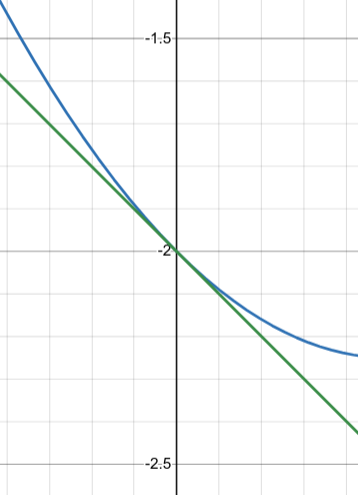
\includegraphics[width=2in]{./resources/tutorial-07-1d.png}

		            It looks like $A_0$ is a good approximation when $-0.12\leq y\leq 0.12$.

		      \item The general solution to $y'=-y-2$ is $y(t)=Ae^{-t}-2$. To find $A$ we plug in our initial
		            condition to get
		            \[
			            y_{\text{approx}}(t)=2e^{-t}-2.
		            \]

		      \item $y_{\text{approx}}$ should be a good approximation of the solution to Equation (A) as long as
		            $-0.12 \leq y_{\text{approx}}(t)\leq 0.12$. By using the formula for $y_{\text{approx}}$,
		            we find this is when $-0.058\leq t \leq 0.06$.
		      \item In the figure below, you can see the solution to Equation (A) in solid blue and $y_{\text{approx}}$ in dashed orange.

		            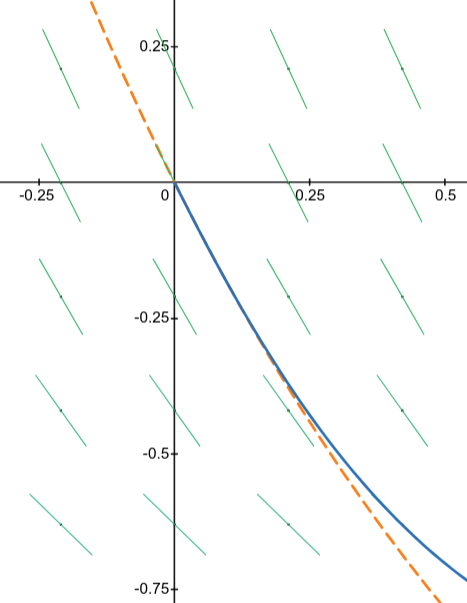
\includegraphics[width=2in]{./resources/tutorial-07-1g.png}

		            It looks like $y_{\text{approx}}$ stops being a good approximation around $t=0.18$, which means
		            that it is a much better approximation than we expected.

		      \item The equilibrium solutions are $y=-1$ and $y=2$.

		            \textbf{Case $y=-1$:}

		            We have an approximation $A_{-1}(y) = -3y-3$. The differential equation $y'=A_{-1}(y)=-3y-3$ has
		            an \emph{attracting} and \emph{stable} equilibrium solution $y=-1$, and so the equilibrium solution
		            for Equation (A) at $y=-1$ is \emph{attracting} and \emph{stable}.

		            \textbf{Case $y=2$:}

		            We have an approximation $A_{2}(y) = 3y-6$. The differential equation $y'=A_{2}(y)=3y-6$ has
		            a \emph{repelling} and \emph{unstable} equilibrium solution $y=2$, and so the equilibrium solution
		            for Equation (A) at $y=2$ is \emph{repelling} and \emph{unstable}.
	      \end{enumerate}
	\item \begin{enumerate}
		      \item Equation (B) cannot be written in matrix or affine form.
		      \item
		      \item The equilibrium solution at $\mat{-1\\1}$ appears to be attracting.
		      \item The total derivative of $\vec F$ at $\mat{-1\\1}$ can be expressed by the matrix
		            \[
			            \mat{-1&0\\-2&-1}.
		            \]
		      \item \[
			            \vec A(x,y) = \mat{-1&0\\-2&-1}\left(\mat{x\\y}-\mat{-1\\1}\right)
		            \]
		      \item We see the eigenvalue of $\mat{-1&0\\-2&-1}$ is $-1$ with geometric and algebraic multiplicity $2$.
		            Therefore its unique equilibrium solution is \emph{stable} and \emph{attracting}.
		      \item Since $\vec A$ is an affine approximation to $\vec F$ at $\mat{-1\\1}$, we know the nature
		            of the equilibrium solution at $\mat{-1\\1}$ should be the same for both $\vec r\,'=\vec F(\vec r)$
		            and $\vec r\,'=\vec A(\vec r)$ (provided that the real part of each eigenvalue is non-zero).
		            Since $\vec r\,'=\vec A(\vec r)$ has a stable and attracting equilibrium solution at $\mat{-1\\1}$,
		            so does $\vec r\,'=\vec F(\vec r)$.

		      \item The remaining equilibrium solutions are $\vec r(t)=\mat{\sqrt{2}\\2}$ and $\vec r(t)=\mat{-\sqrt{2}\\2}$.
		            After linearizing at $\mat{\sqrt{2}\\2}$ and $\mat{-\sqrt{2}\\2}$, we find that both equilibrium solutions
		            are \emph{unstable} but not \emph{repelling} (the corresponding matrices have a mix of one positive and one negative eigenvalue).

	      \end{enumerate}
\end{enumerate}
	
	\end{solutions}
	\begin{instructions}
		\subsection*{Learning Objectives}
Students need to be able to\ldots
\begin{itemize}
	\item Create affine approximations to a differential equations
	\item Use affine approximation to determine the stability of equilibrium solutions
	\item Recognize that affine approximations are still approximations even when not centered at an equilibrium solution
\end{itemize}

\subsection*{Context}
In lecture, students have linearized a 1d differential equation and used it to analyze the stability of equilibrium solutions.
We have also done this \emph{one time} for a 2d system. 1d affine approximations are familiar to the students from Calc I,
but 2d affine approximations are new to them (though everyone should be taking or have already taken multivariable calculus at this point).

\subsection*{What to Do}
Start the tutorial by stating the day's learning objectives. There is one focus: understand
how to find affine approximations to differential equations and what those affine approximations tell us.

Have everyone get into groups and start on \#1. This will take most students most of the time. If they
do finish \#1, \#2 will take all the remaining time.

6 minutes before the end of class, pick a suitable problem to do as a wrap-up. Unless everyone has finished \#1,
picking one equilibrium for 1h is probably a good choice.

\subsection*{Notes}
\begin{enumerate}
	\item The first several parts of this question focus on an affine approximation \emph{away} from an equilibrium solution.
	      This is on purpose.
	      \begin{enumerate}
		      \item
		      \item Most of the equilibrium solutions we study in this class are at the origin, but not this time. This question
		            is a sanity check to see if students have any idea about what is going on in the course at this point. Most students
		            should have a quick answer to this question. If they don't force them to think about it---they shouldn't be skipping it!
		      \item If they struggle, prod them to think about ``linear approximations'' from Calculus, or about tangent lines.
		      \item Many will choose the vertical axis as the ``$y$'' axis. It is the horizontal axis in this case.
		      \item If they struggle, remind them it is separable.
		      \item Judgement call for the student. Their estimation will be wrong anyways, but making guesses is always a good thing!
		      \item This should be \emph{very} routine for them at this point. To copy-and-paste into Desmos, you must omit the header
		            columns from the spreadsheet.
		      \item They have to put all their knowledge together in this part. If they get stuck, encourage them to work through the
		            previous steps replacing $y=0$ with an equilibrium solution they found.

	      \end{enumerate}
	\item Only the quick students will make it this far. It basically mimics \#1 but in 2d and starting with an equilibrium point
	      rather than some random point.
\end{enumerate}
	\end{instructions}

\end{document}
